%!TEX root = ../../report.tex
\chapter{Results} % (fold)
\label{cha:results}
The main result of this project-oriented thesis is the first prototype of the bipedal platform for human-like locomotion studies RuBi, and its development and study environment.
The work carried out for the last four months has comprised from the origin of the idea and its initial conceptualization to the last steps taken on its mechatronics construction, the development of its control and electronics architecture, its simulation model and environment and the devise of the tests it should have been subject to in the presence of more time.
The outputs of the whole workflow presented in this report are summarized in this chapter for an overall view of the results, although they have been discussed more in detail in their respective chapters.


\section{Morphological properties of RuBi} % (fold)
\label{sec:rubi_mechanical_properties}
The geometrical and inertial dimensions of the final prototype of RuBi can be found in table \ref{tab:limb_physical_properties}.
The geometry of the robot has been inspired in the lower limbs of a male person in order to facilitate human-like motion for research in this field.
However its inertial properties have been minimized in order to reduce power requirements and their inherent economical aspects (a more powerful powertrain would entail greater costs).
From a mechanical perspective, this has been translated into the application of light but resistant materials, while striving for low cost, standardization and easy maintenance, achieving a low weight and reduced inertias, as can be seen in table \ref{tab:limb_physical_properties}.

A comparison between other two-dimensional bipedal robots of similar morphology to RuBi can be seen in \ref{fig:bipedal_robots}.
It can be easily appreciated that the overall length-weight ratio of RuBi is significantly better than more developed models as the Phides \cite{phides} or BioBiped \cite{biobiped}, even considering that they have an on-board controller and all this implies.

\begin{figure}[h]
\centering
  \begin{subfigure}{.22\textwidth}
    %\centering
    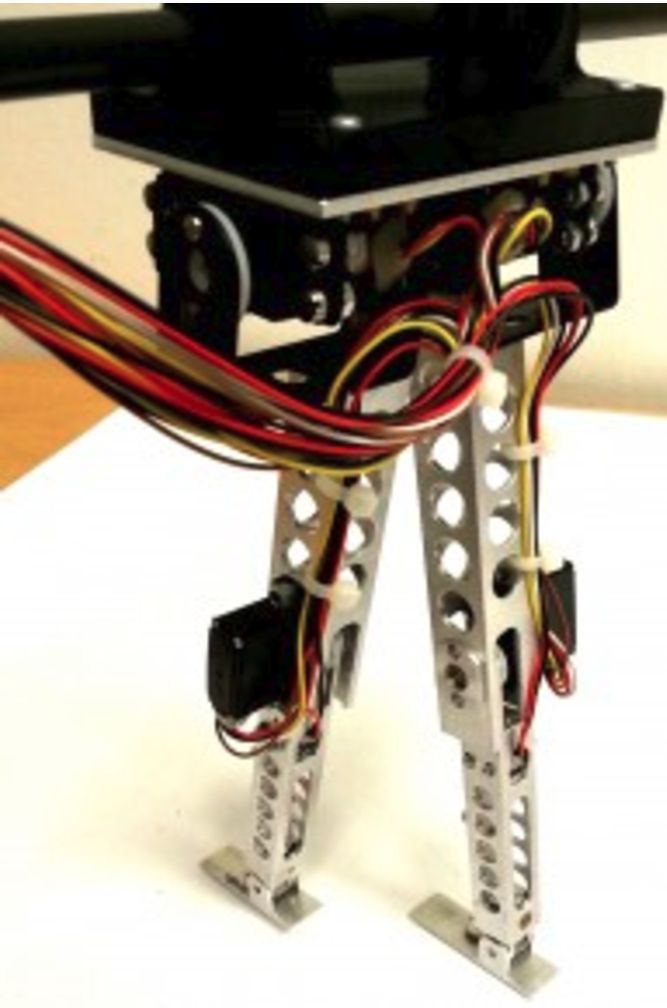
\includegraphics[width=0.9\linewidth]{figures/w_dacbot.pdf}
    \caption{DACbot\\
    Lenght = 0.35m\\
    Weight = 0.58Kg}
    \label{fig:w_dacbot}
  \end{subfigure}
  \begin{subfigure}{.22\textwidth}
    %\centering
    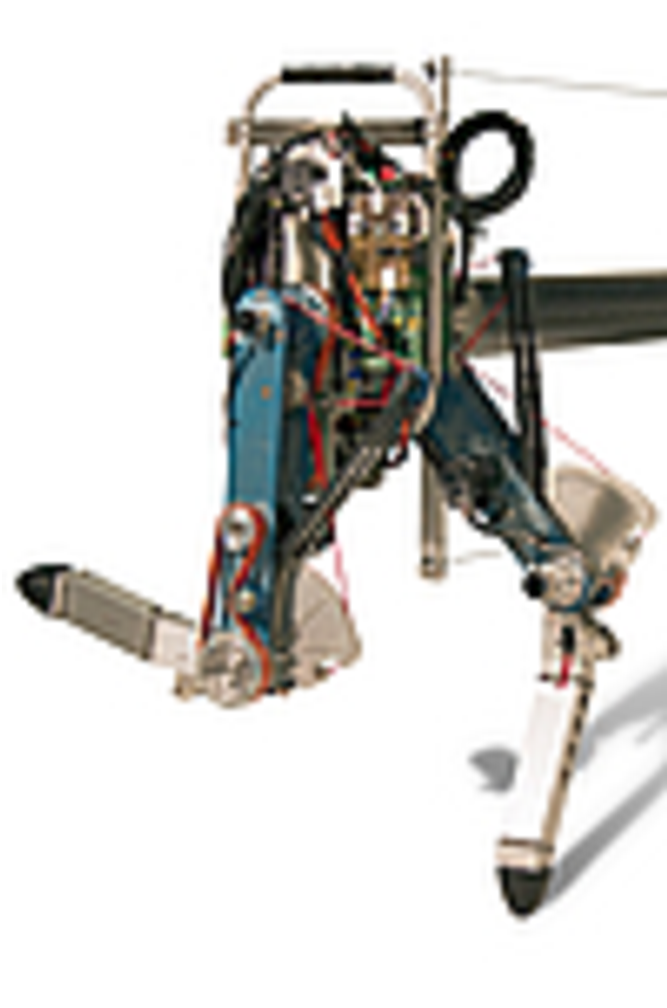
\includegraphics[width=0.9\linewidth]{figures/w_phides.pdf}
    \caption{Phides\\
    Lenght = 0.8m\\
    Weight = 13.5Kg}
    \label{fig:w_phides}
  \end{subfigure}
  \begin{subfigure}{.22\textwidth} 
    %\centering
    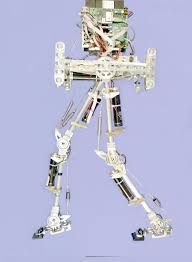
\includegraphics[width=\linewidth]{figures/w_biobiped.jpg}
    \caption{BioBiped\\
    Lenght = 1.1m\\
    Weight = 10Kg}
    \label{fig:w_biobiped}
  \end{subfigure}
  \begin{subfigure}{.22\textwidth}
    %\centering
    \includegraphics[width=0.9\linewidth]{figures/w_RuBi.pdf}
    \caption{RuBi\\
    Lenght = 0.57m\\
    Weight = 0.71Kg}
    \label{fig:w_rubi}
  \end{subfigure}
  \caption{Length-weight comparative with existing bipeds}
  \label{fig:bipedal_robots}
\end{figure}  


\begin{table}[htbp]
\caption{Physical properties of the limbs obtained from CAD program}
\begin{center}
\begin{tabular}{c|c|c|c}
 \vspace{5mm}
\large \textbf{Limb} & \large  \textbf{Length [$m$]} & \large  \textbf{Mass [$Kg$]} & \large \textbf{Moments of inertia [$Kg \cdot m^2$]} \\

Foot & 0.095 & 0.021 & \vspace{5mm} \begin{tabular}{c|c|c}
                        2.2e-005 & -9.16e-006 & 0 \\ \hline
                        -9.16e-006 & 9.05e-006 & 0 \\ \hline
                        0 & 0 & 2.88e-005 
                        \end{tabular} \\
Lower limb & 0.115 & 0.2 & \vspace{5mm} \begin{tabular}{c|c|c}
                        0.000699 & 2.44e-005 & 0 \\ \hline
                        2.44e-005 & 1.85e-005 & -1.82e-005 \\ \hline
                        0 & -1.82e-005 & 0.000694
                        \end{tabular}\\ 

Upper limb & 0.123 & 0.2 & \vspace{5mm} \begin{tabular}{c|c|c}
                        0.00119 & 2.89e-006 & -1.36e-008 \\ \hline
                        2.89e-006 & 1.69e-005 & -1.78e-005 \\ \hline
                        -1.36e-008 & -1.78e-005 & 0.00118
                        \end{tabular}\\
Hip & 0.150 & 0.156 & \vspace{5mm} \begin{tabular}{c|c|c}
                        0.000303 & 0 & 1.44e-008 \\ \hline
                        0 & 2.78e-005 & 0 \\ \hline
                        1.44e-008 & 0 & 0.000314
                        \end{tabular}\\ 
Total & & 0.707 &
\end{tabular}
\end{center}
\label{tab:limb_physical_properties}
\end{table}

\todo{Add theoretical froude number?}

% section rubi_mechanical_properties (end)

\section{Actuation and sensory feedback} % (fold)
\label{sec:actuation_and_sensory_feedback}
RuBi has six actuated joints for planar motion.
For each of them, a fully functional and extendable embedded electronics system based on the Locokit hardware has been implemented as the spinal cord of the robot, together with a software interface able to handle the information flow with the robot.
It provides access to the angular information of each joint in real time and the control of their individual torque commands, all through a standard ROS interface that can be used as well for controlling the simulation model.
As an example, the readings from hip, knee and ankle encoders for a random movement on one leg are shown in Figure \ref{fig:position_measurements}.


\begin{figure}[h]
  \centering
  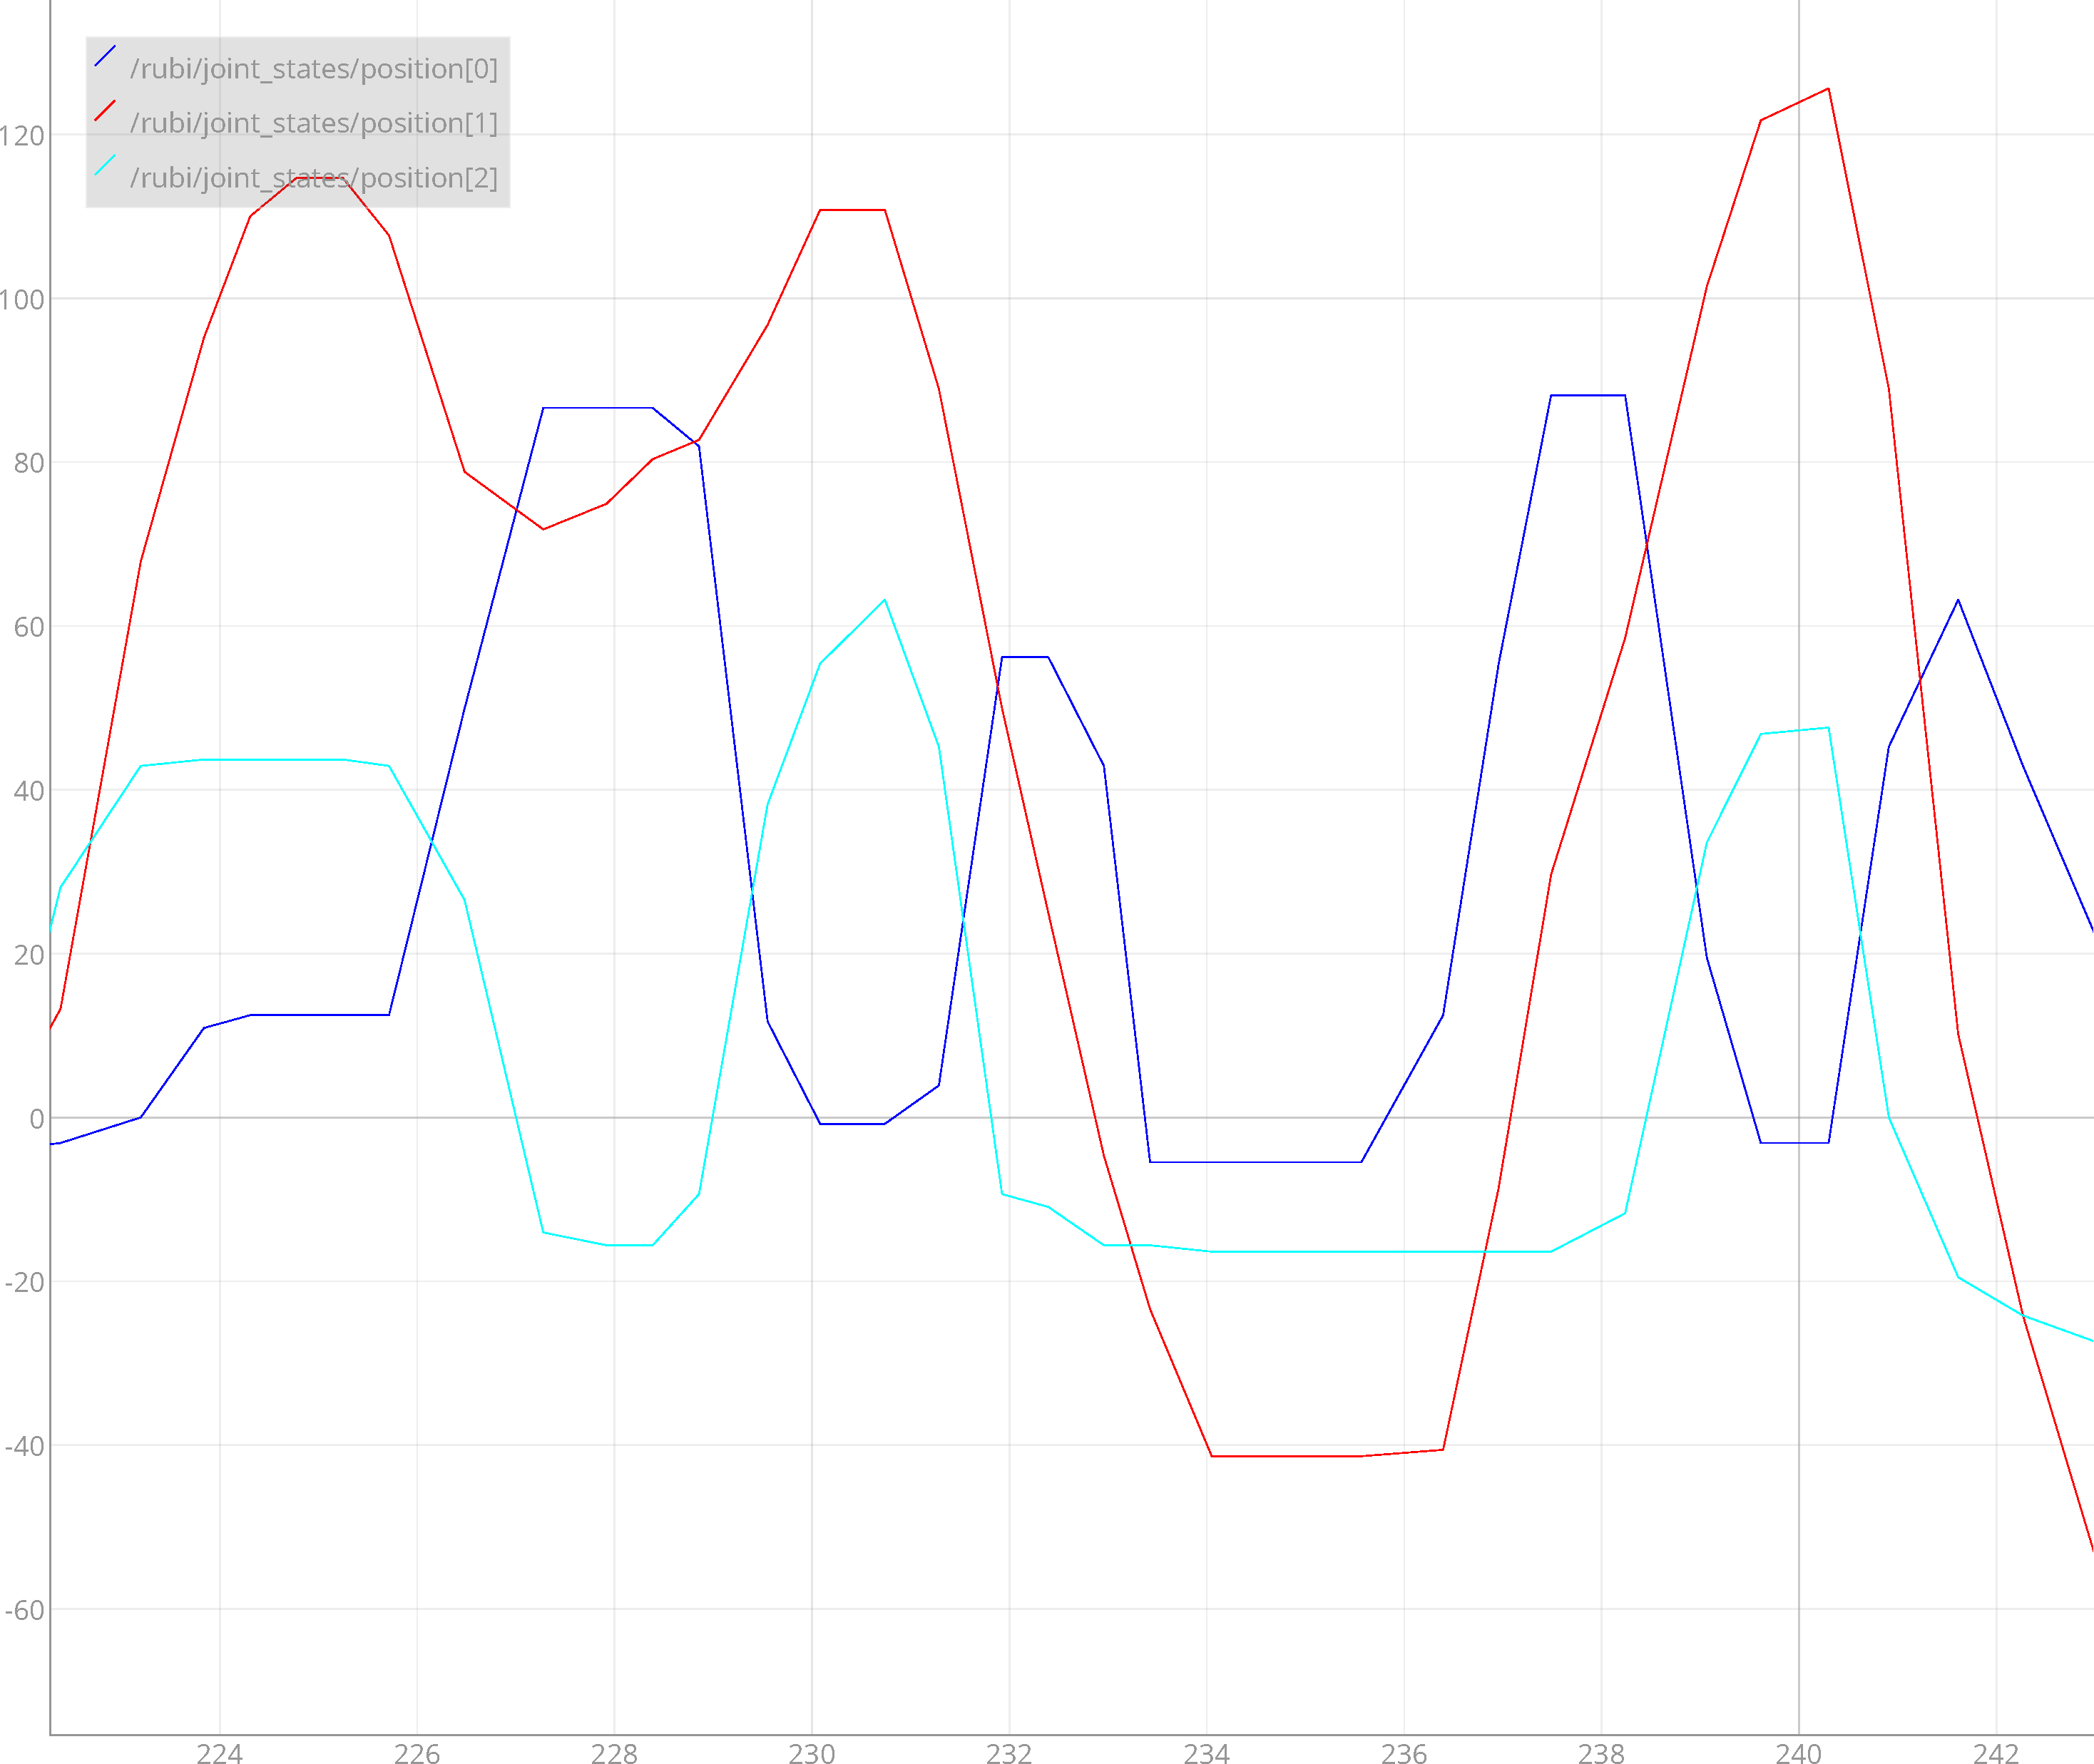
\includegraphics[width=0.7\textwidth]{figures/position_measurements.pdf}
  \caption{Measurements obtained from real robot}
  \label{fig:position_measurements}
\end{figure}


The six actuators on the robot has been individually tested once on-board although detached of the transmissions due to the delay on the delivery of the springs explained.
Its selection has been based on the calculations introduced in Algorithm 1 detailed in \ref{sub:electric_actuators}, that have made use of the dynamic model of the robot constructed.

All the control hardware has been placed off-board to reduce weight on the frame.

Contact sensors have been placed on the heels of the robot to offer the possibility of monitoring ground contact during the locomotion.
However, they have not been connected to the electronics frame due to unforeseen issues with the hardware frame, that could be easily overcome with simple additional circuitry and some more time.
% section actuation_and_sensory_feedback (end)

\section{RuBi dynamic model and actuators calculation} % (fold)
\label{sec:rubi_dynamic_model_and_actuators_calculation}
The MATLAB scripts containing the implementation and results of the dynamic model of the robot and the calculus for the parameters of the actuators can be found in the source folder attached to this thesis.
The final model has been considered a fair trade-off between simplicity and accuracy, since the addition of more terms hard to model as frictions or backslash in the transmissions would not have contributed additional value.

Section \ref{sec_dynamic_controller} has presented a possible intrinsic use of the dynamic model of the robot, which is to conduct torque control on the robot through its real-time computation. 
However, the application of the model as a controller has not been fully developed and it is just left in this report as a proof of concept and to suggest its potential use.
% section rubi_dynamic_model_and_actuators_calculation (end)


\section{Framework for experimentation} % (fold)
\label{sec:framework_for_experimentation}
A novelty of RuBi is the possibility of implementing four different elastic actuation configurations in each knee and ankle joint.
SEA, PEA, SEA+PEA and DD configurations can be utilized for the transmission of the motion to the joints.
This converts RuBi into an ideal platform to study the influence of the compliance configuration on the energy storage capacity of a bipedal platform or on the power peak consumption of the joints, for instance.

For facilitating the conduction of locomotion experiments, a test bench that allows a fully controlled 2D legged motion for the robot has been built on the top of a treadmill.
It can be easily modified to be used for hopping or jumping motion experimentation.
Some experiments devised for testing the prototype are suggested in \ref{cha:experiments} although not carried out due to time constraints and delays suffered.
% section framework_for_experimentation (end)

\section{Simulation environment} % (fold)
\label{sec:simulation_environment}
A simple and extendable simulation environment together with a robot model have been created in Gazebo.
The physical properties of the robot and its visual model have been exported from its design in SolidWorks for maximum resemblance with the real device.
A ROS interface has been created for the simulation environment, together with two simple controllers that have been successfully tested (see \ref{cha:experiments}).
They have been used also to prove the simplicity of the development and testing of control algorithms with the simulation model.
In Figure \ref{fig:RuBi_jump_sequence} a sequence of snapshots depicts RuBi performing an unconstrained jump as a result of the use of the impulse controller in the simulation.
It has been used to demonstrate that the physical characteristics of the structure are capable of handle the motion implied in a jump. 
\begin{figure}[ht!]
    \centering
    \begin{subfigure}[b]{0.16\textwidth}
        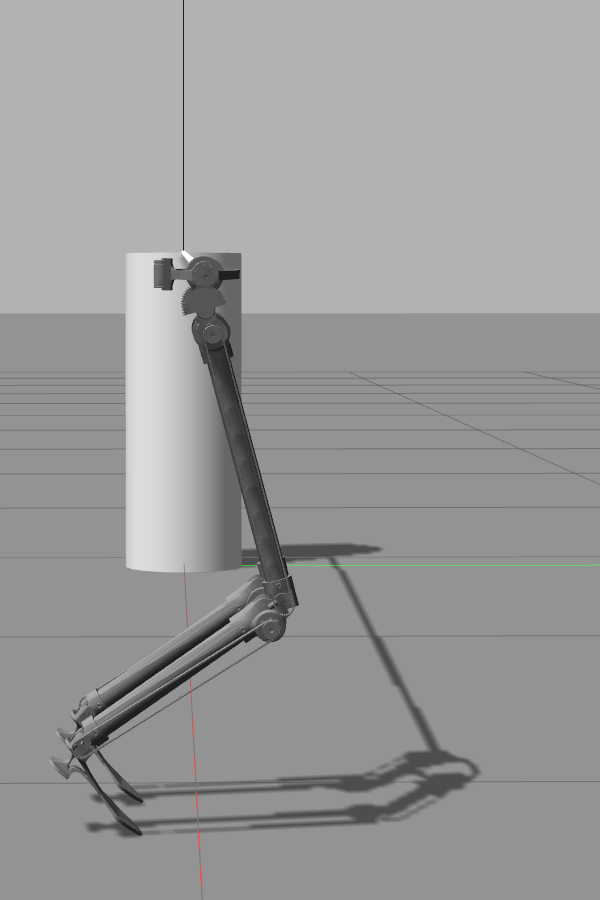
\includegraphics[width=\textwidth]{figures/gazebo_jumping_1}
    \end{subfigure}
    \begin{subfigure}[b]{0.16\textwidth}
        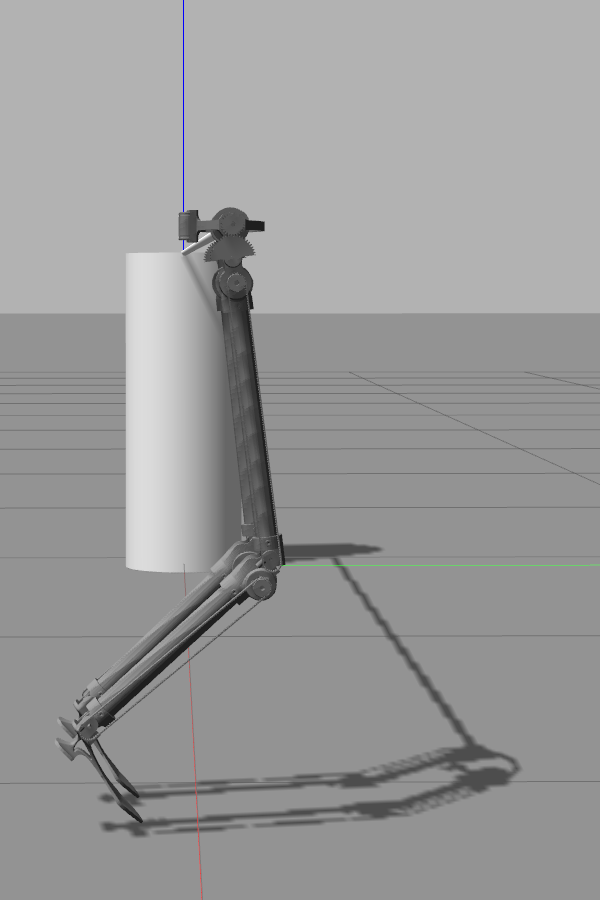
\includegraphics[width=\textwidth]{figures/gazebo_jumping_2}
    \end{subfigure}
    \begin{subfigure}[b]{0.16\textwidth}
        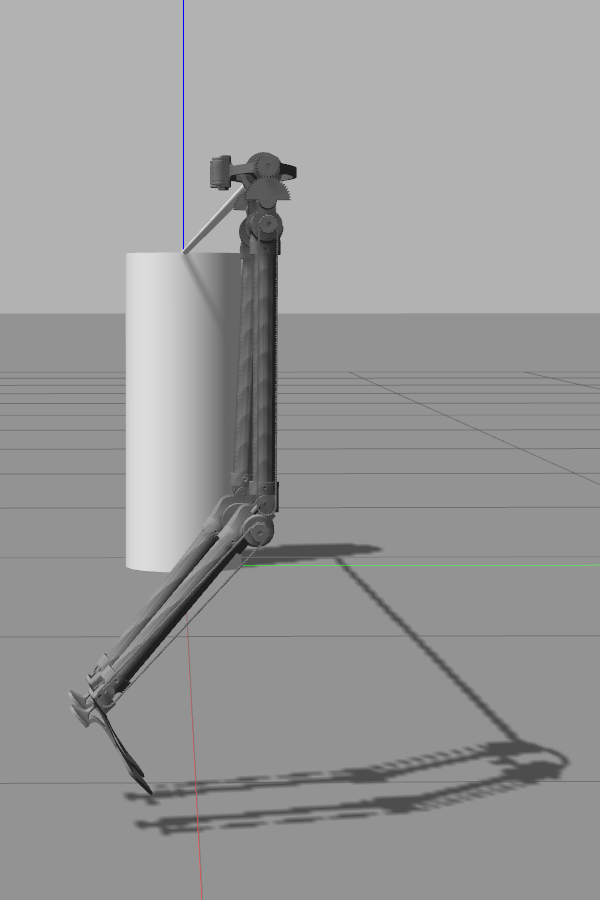
\includegraphics[width=\textwidth]{figures/gazebo_jumping_3}
    \end{subfigure}
    \begin{subfigure}[b]{0.16\textwidth}
        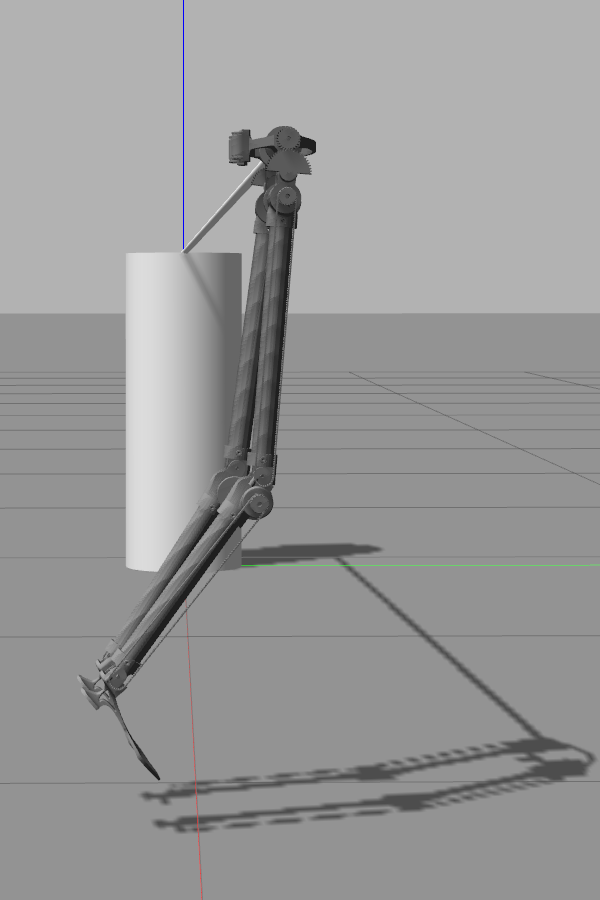
\includegraphics[width=\textwidth]{figures/gazebo_jumping_4}
    \end{subfigure}
    \begin{subfigure}[b]{0.16\textwidth}
        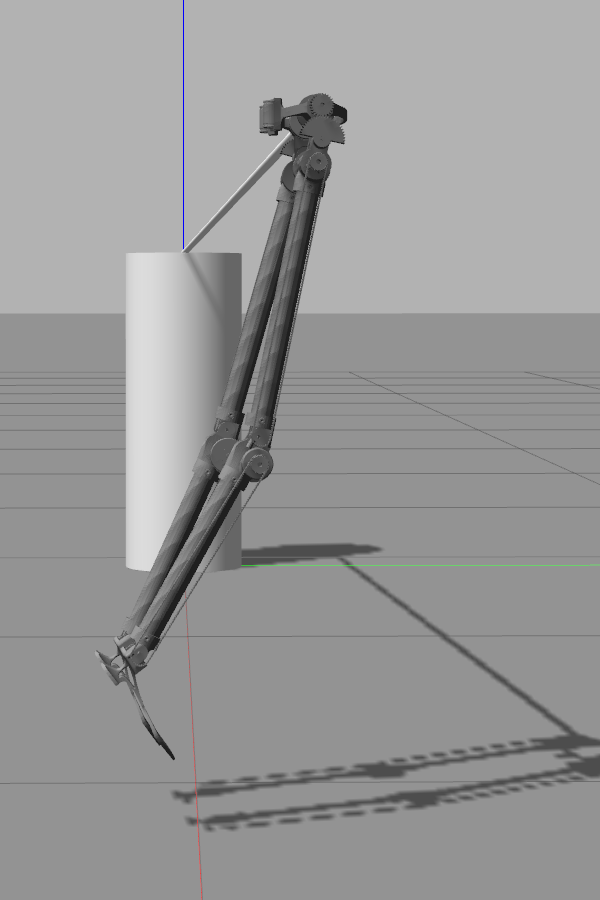
\includegraphics[width=\textwidth]{figures/gazebo_jumping_5}
    \end{subfigure}
    \begin{subfigure}[b]{0.16\textwidth}
        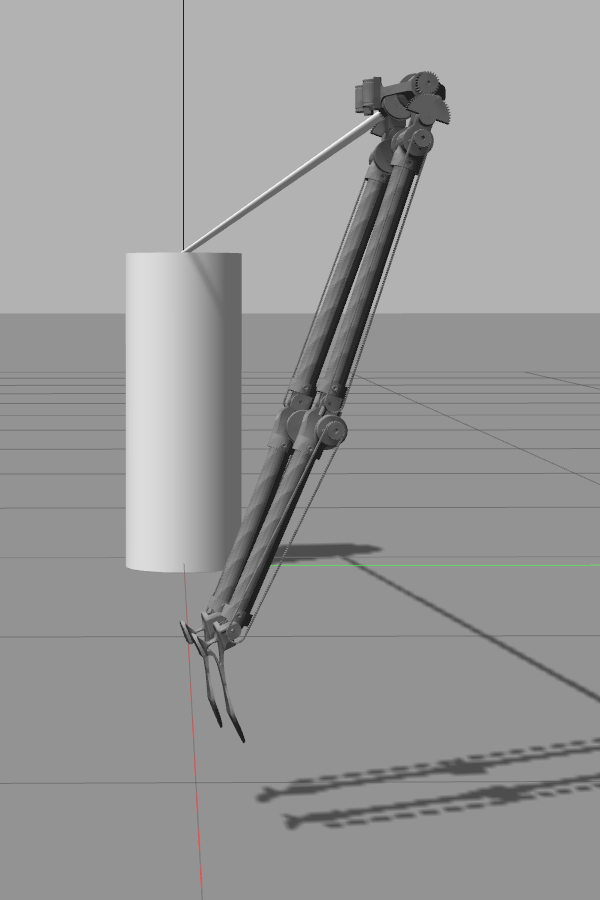
\includegraphics[width=\textwidth]{figures/gazebo_jumping_7}
    \end{subfigure}
    \caption{Snapshots of RuBi performing an unconstrained jump}
    \label{fig:RuBi_jump_sequence}
\end{figure}      

However, the problems of the physics engine to handle robots of the size of RuBi led to the need of truncating some of its too small physical properties in order to be able to simulate real behaviors.
Hence, the simulation model can be used to qualitatively test the functionality of controllers, but their outputs will have to be adapted to the real environment until the simulation model is further improved.
% section simulation_environment (end)


% chapter results (end)